I conduct extensive analysis to better understand my models in terms
of learning, the ability to handle long sentences, 
choices of attentional architectures, and alignment quality. All results
reported here are on English-German newstest2014.

\subsection{Learning curves}
I compare models built on top of one another %with the {\it additive} features
%: source reverse, dropout, global attention, input
%feeding, and local attention with predictive alignments. Figure~\ref{f:learn}
%shows that these learning curves well reflect the performances of their
%corresponding models 
as listed in Table~\ref{t:ende}. It is
pleasant to observe in Figure~\ref{f:learn} a clear separation between non-attentional and attentional
models. The input-feeding approach and the local attention
model also demonstrate their abilities in driving the test costs lower. The
non-attentional model with 
dropout (the blue + curve) learns slower than other non-dropout models, but
as time goes by, it becomes more robust in terms of minimizing test errors.
\begin{figure}
\centering
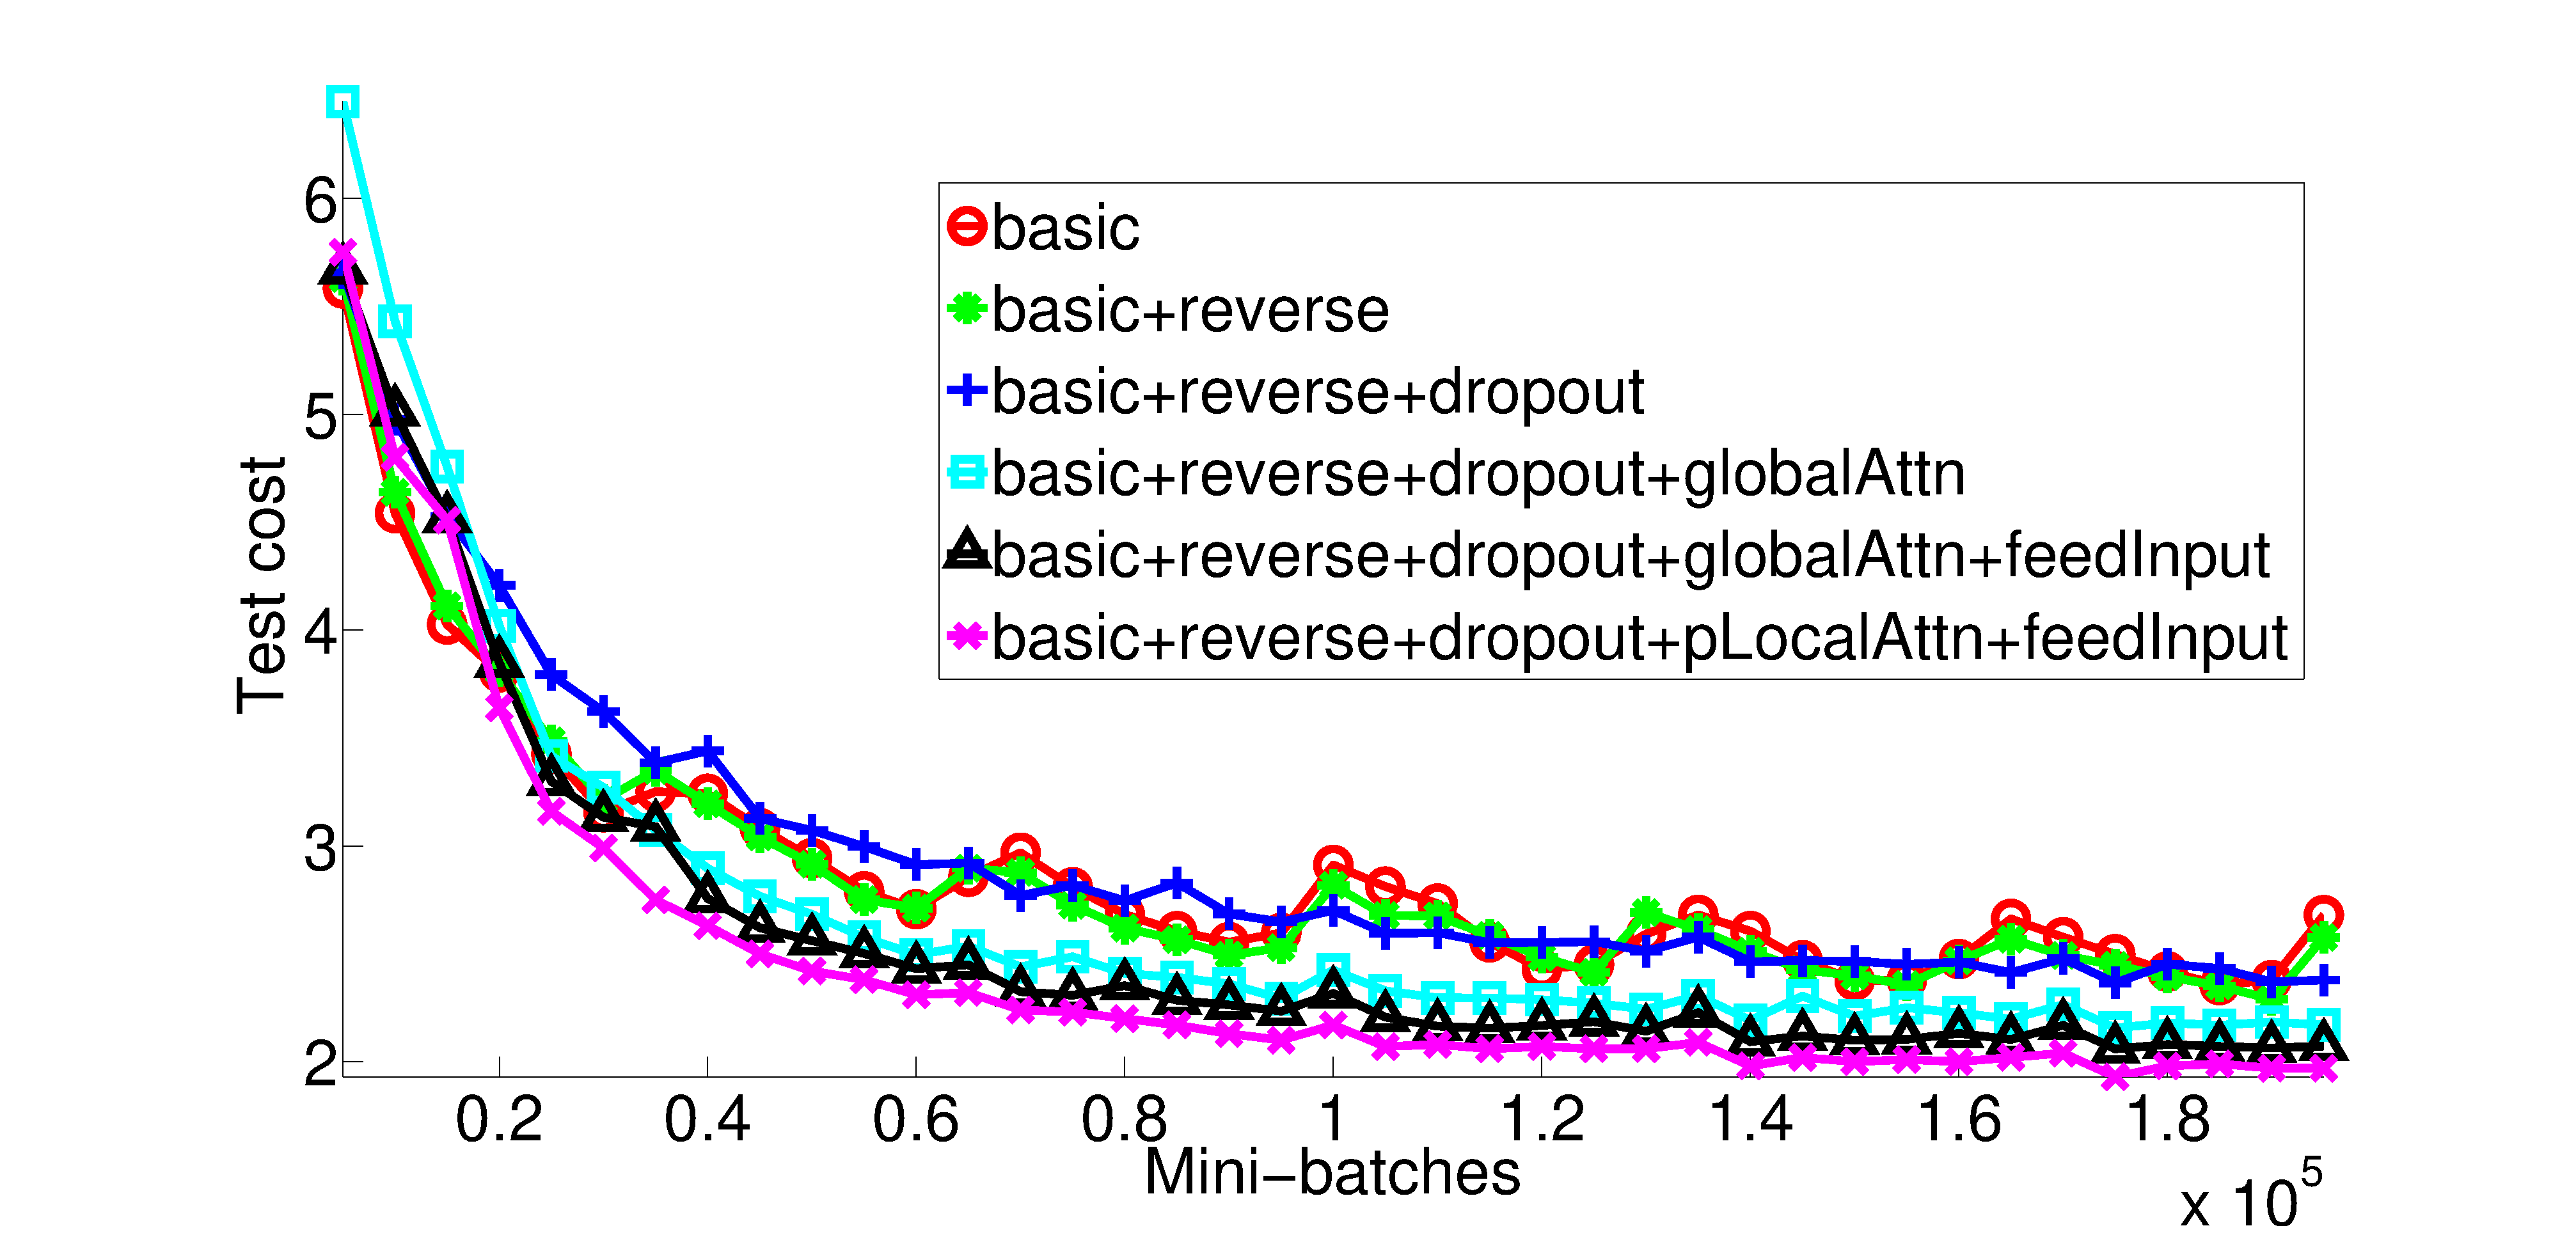
\includegraphics[width=0.7\textwidth, clip=true, trim=140 0 70 0]{img/4-learning} % , angle=-90
\caption[Learning curves]{{\bf Learning curves} -- test cost ($\ln$ perplexity) on newstest2014 for English-German NMTs as training progresses.
} 
\label{f:learn}
\end{figure}

\subsection{Effects of Translating Long Sentences}
I follow \cite{bog15} to group sentences of similar lengths together and
compute a BLEU score per group. Figure~\ref{f:length} shows that
my attentional models are more effective than the non-attentional one in
handling long sentences: the quality does not degrade as sentences
become longer. My best model (the blue + curve) outperforms all other systems in all length buckets.

\begin{figure}[tbh!]
\centering
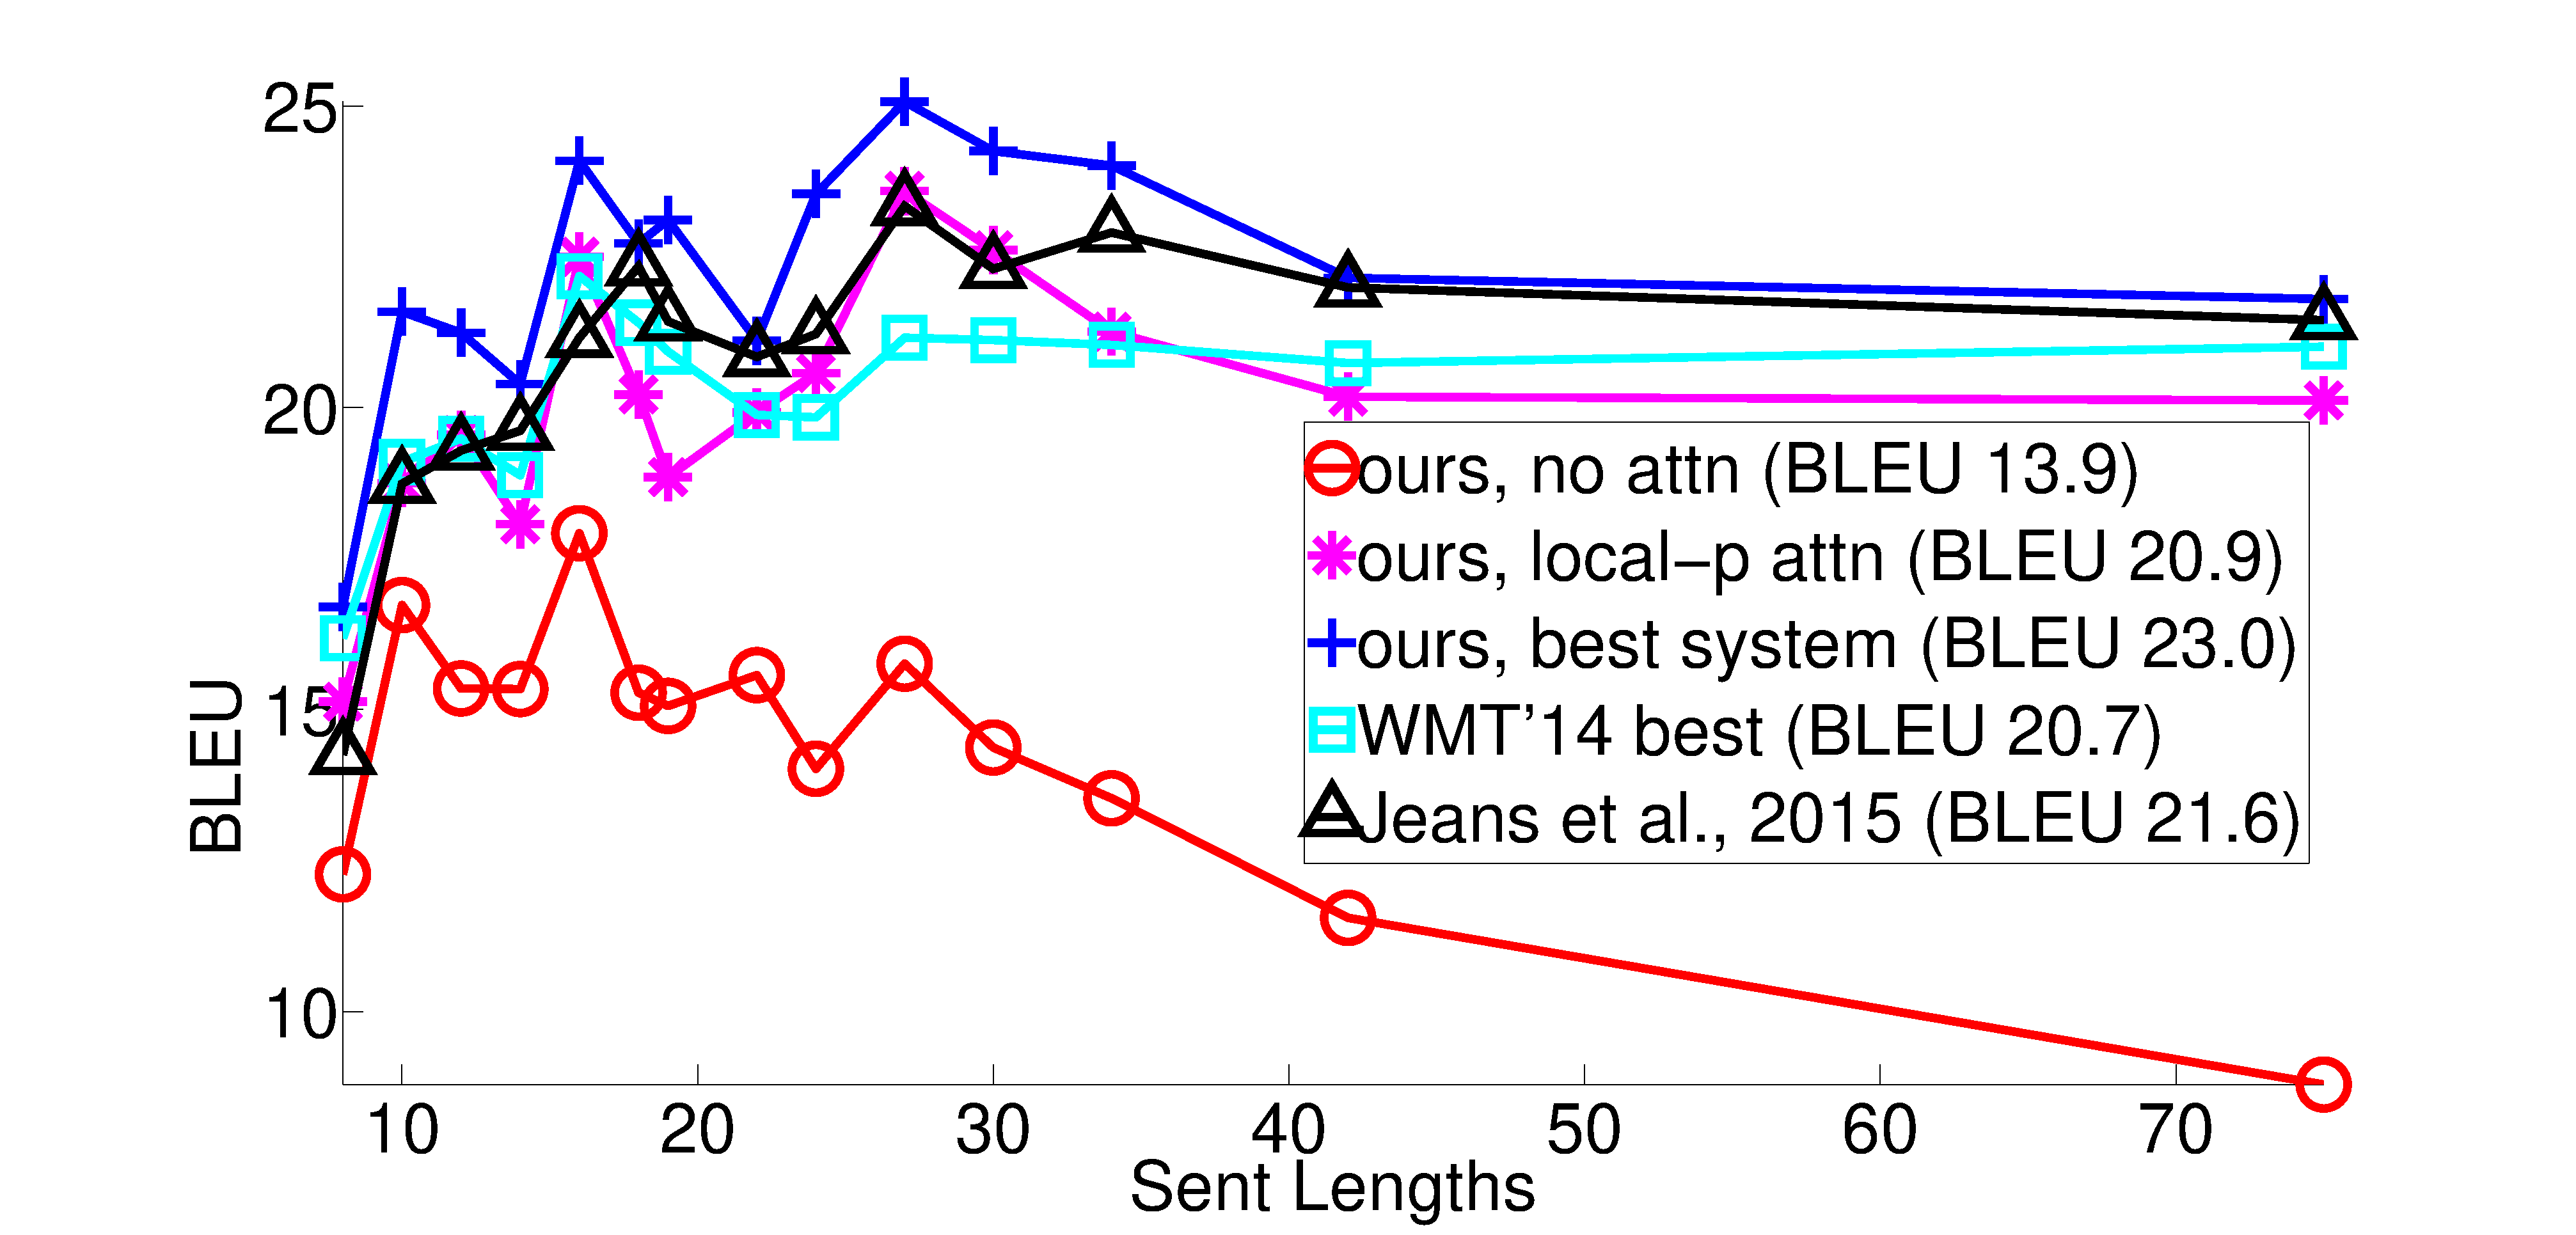
\includegraphics[width=0.7\textwidth, clip=true, trim=120 0 70 0]{img/4-length} % , angle=-90
\caption[Length Analysis]{{\bf Length Analysis} -- translation qualities of different
systems as sentences become longer.
} 
\label{f:length}
\end{figure}

\subsection{Choices of Attentional Architectures}
I examine different attention models ({\it global, local-m, local-p}) and different
alignment functions ({\it location, dot, general, concat}) as described in
Section~\ref{sec:attn}. Due to limited
resources, I cannot run all the possible combinations.
However, results in Table~\ref{t:attnChoices} do give us some idea about
different choices. 
The {\it location-based} function does not learn good
alignments: the {\it global (location)} model can only obtain a small
gain when performing unknown word replacement compared to using other alignment
functions.\footnote{There is a subtle difference in how I retrieve alignments
for the different alignment functions. At time step $t$ in which I receive
$\tgt{t-1}$ as input and then compute $\hi, \al, \co$, and $\hs$ before
predicting $\tgt{t}$, the alignment vector $\al$ is used as alignment
weights for (a) the predicted word $\tgt{t}$ in the {\it location-based}
alignment functions and (b) the input word $\tgt{t-1}$ in the {\it content-based}
functions.}
For {\it content-based} functions, my implementation {\it concat} does not yield good performances
and more analysis should be done to understand the
reason.\footnote{With {\it concat}, the perplexities achieved by different models are 6.7 (global), 7.1
(local-m), and 7.1 (local-p). Such high perplexities could be due to the fact
that I simplify the matrix \MB{W_a} to set the part that corresponds to $\his$
to identity.} It is interesting to observe that {\it dot} works
well for the global attention and {\it general} is better for the local
attention.
Among the different models, the local attention model with predictive alignments ({\it
local-p}) is best, both in terms of perplexities and BLEU.

\begin{table}
\centering
%\resizebox{8cm}{!}{
\begin{tabular}{l|r|c|c}
\multirow{ 2}{*}{\bf{System}} & \multirow{ 2}{*}{\bf{Ppl}} &
\multicolumn{2}{c}{{\bf BLEU}}\\
\cline{3-4}
& & Before & After unk \\
  \hline
global (location) & 6.4 & 18.1 & 19.3 (+1.2) \\
%global (concat) & 6.7 & xx & xx (+xx) \\
global (dot) & 6.1 & 18.6 & 20.5 (+1.9) \\
global (general) & 6.1 & 17.3 & 19.1 (+1.8) \\
  \hline
local-m (dot) & $>$7.0 & x & x \\
local-m (general) & 6.2 & 18.6 & 20.4 (+1.8) \\
  \hline
local-p (dot) & 6.6 & 18.0 & 19.6 (+1.9) \\
local-p (general) & {\bf 5.9} & {\bf 19} & {\bf 20.9 (+1.9)} \\
\end{tabular}
%}
\caption[Attentional Architectures]{{\bf Attentional Architectures} -- performances of different
attentional
models. I trained two local-m (dot) models; both have
ppl $>7.0$.}
\label{t:attnChoices}
\end{table}

\subsection{Alignment Quality}
A by-product of attentional models are word alignments. While \cite{bog15}
visualized alignments for some sample sentences and 
observed gains in translation quality as an indication of a working attention
model, no work has assessed the alignments learned as a whole. In contrast, I
set out to evaluate the alignment quality using the alignment error rate (AER)
metric.

\begin{table}
  \begin{center}
    \begin{tabular}{c c}
      {\bf Method} & {\bf AER} \\
      \hline
      global (location) & $0.39$ \\
      local-m (general)  & $0.34$ \\
      local-p (general) & $0.36$ \\
      \hdashline
      ensemble & $0.34$ \\
      \hline
      Berkeley Aligner & $0.32$ \\
    \end{tabular}
  \end{center}
  \caption[AER scores]{{\bf AER scores} -- results of various models on the RWTH
  English-German alignment data.}
  \label{t:alignment}
\end{table}

Given the gold alignment data provided by RWTH for 508 English-German
Europarl sentences, I ``force'' decode my attentional models to
produce translations that match the references. I extract only one-to-one
alignments by selecting the source word with the highest alignment
weight per target word. Nevertheless, as shown in Table~\ref{t:alignment}, I were able to achieve AER scores
comparable to the one-to-many alignments obtained by the Berkeley aligner
\cite{liang06alignment}.\footnote{I concatenate the 508 sentence pairs with 1M
sentence pairs from WMT and run the Berkeley aligner.}

I also found that the alignments produced by local attention models achieve
lower AERs than those of the global one. The AER obtained by the ensemble, while
good, is not better than the local-m AER, suggesting the well-known
observation that AER and translation scores are not well correlated \cite{fraser07}.
%Due to space constraint, we can only show alignment visualizations in the arXiv version of our
%paper.\footnote{\url{http://arxiv.org/abs/1508.04025}}
%We show some alignment visualizations in Appendix~\ref{sec:visual}.

\subsection{Sample Translations}
\label{sec:sample}
I show in Table~\ref{t:sample} sample translations in both directions. It it
appealing to observe the effect of attentional models in correctly translating
names such as ``Miranda Kerr'' and ``Roger Dow''. Non-attentional models, while producing sensible names from a language
model perspective, lack the direct connections from the source side to make
correct translations. % as with the case of attention-based NMT systems. 
I also observed an interesting case in the second
example, which requires translating the {\it doubly-negated} phrase, ``not incompatible''.
The attentional model correctly produces ``nicht $\dots$ unvereinbar'';
whereas the non-attentional model generates ``nicht vereinbar'', meaning
``not compatible''.\footnote{The reference uses a more fancy translation of
``incompatible'', which is ``im Widerspruch zu etwas stehen''. Both models, however, failed to translate ``passenger
experience''.} The attentional
model also demonstrates its superiority in translating long sentences as in
the last example.
\begin{table*}[tbh!]
\centering
\resizebox{15cm}{!}{
\begin{tabular}{c|p{15cm}}
\multicolumn{2}{l}{{\bf English-German translations}}\\
  \hline
src & Orlando Bloom and Miranda Kerr still love each other \\
  \hline
ref & Orlando Bloom und \correct{Miranda Kerr} lieben sich noch immer \\
  \hline
{\it best} & Orlando Bloom und \correct{Miranda Kerr} lieben einander noch immer . \\
  \hline
base & Orlando Bloom und \wrong{Lucas Miranda} lieben einander noch immer .\\
  \hline
  \hline
src & $''$ We $'$ re pleased the FAA recognizes that an enjoyable passenger experience is not incompatible with safety and security , $''$ said Roger Dow , CEO of the U.S. Travel Association . \\
  \hline
ref & `` Wir freuen uns , dass die FAA erkennt , dass ein angenehmes
Passagiererlebnis nicht im Widerspruch zur Sicherheit steht '' , sagte
\correct{Roger Dow} , CEO der U.S. Travel Association . \\
  \hline
{\it best} & $''$ Wir freuen uns , dass die FAA anerkennt , dass ein angenehmes ist
nicht mit Sicherheit und Sicherheit \correct{unvereinbar} ist $''$ , sagte \correct{Roger
Dow} , CEO der US - die . \\
  \hline
base & $''$ Wir freuen uns \"{u}ber die $<$unk$>$ , dass ein $<$unk$>$ $<$unk$>$
mit Sicherheit nicht \wrong{vereinbar} ist mit Sicherheit und Sicherheit $''$ ,
sagte \correct{Roger} \wrong{Cameron} , CEO der US - $<$unk$>$ . \\
  \hline
  \hline
\multicolumn{2}{l}{{\bf German-English translations}}\\
  \hline
src & In einem Interview sagte Bloom jedoch , dass er und Kerr sich noch immer lieben . \\
  \hline
ref & However , in an interview , Bloom has said that he and \correct{Kerr} still love each other . \\
  \hline
{\it best} & In an interview , however , Bloom said that he and \correct{Kerr} still love . \\
  \hline
base & However , in an interview , Bloom said that he and \wrong{Tina} were still $<$unk$>$ . \\
  \hline
  \hline
src & Wegen der von Berlin und der Europ\"{a}ischen Zentralbank verh\"{a}ngten strengen Sparpolitik in Verbindung mit der Zwangsjacke , in die die jeweilige nationale Wirtschaft durch das Festhalten an der gemeinsamen W\"{a}hrung gen\"{o}tigt wird , sind viele Menschen der Ansicht , das Projekt Europa sei zu weit gegangen \\ 
  \hline
ref & The \correct{austerity imposed by Berlin and the European Central Bank , coupled with the straitjacket} imposed on national economies through adherence to the common currency , has led many people to think Project Europe has gone too far .\\
  \hline
{\it best} & Because of the strict \correct{austerity measures imposed by Berlin
and the European Central Bank in connection with the straitjacket} in which the
respective national economy is forced to adhere to the common currency , many
people believe that the European project has gone too far . \\
  \hline
base & Because of the pressure \wrong{imposed by the European Central Bank and the Federal Central Bank with the strict austerity} imposed on the national economy in the face of the single currency , many people believe that the European project has gone too far .\\
\end{tabular}
}
\caption[Sample translations]{{\bf Sample translations} -- %examples in both translation directions.
for each example, I show the source ({\it src}), the human translation ({\it
ref}), the translation from my best model ({\it best}), and the
translation of a non-attentional model ({\it base}).  I italicize some
\correct{correct} translation segments and highlight a few \wrong{wrong} ones in
bold.} % See Appendix~\ref{sec:sample} for detailed descriptions.}
\label{t:sample}
\end{table*}



